\documentclass{beamer}
\usetheme{Madrid}
\setbeamertemplate{bibliography item}{}

\usepackage{listings}
\newcommand*{\code}[1]{\lstinline[basicstyle=\ttfamily, breaklines]|#1|}

\usepackage{graphicx}
\usepackage{svg}
\usepackage{caption}
\svgsetup{inkscapepath=build/svg-inkscape/}
\graphicspath{{figure/}}

\title[MiniSatUP and its Integration with cvc5]{From MiniSat to MiniSatUP and its Integration \\ with cvc5 via IPASIR-UP}
\author{Chenqi Hao}
\institute{University of Freiburg}
\date{\today}

\begin{document}

\begin{frame}
  \centering \textit{Master's Thesis}
  \titlepage
  \centering {
    \small
    \begin{tabular}{ll}
      Advisor: & Prof. Dr. Armin Biere (University of Freiburg) \\
      & Assistant Prof. Dr. Katalin Fazekas (TU Wien) \\
      Co-advisor: & Dr. Mathias Fleury (University of Freiburg)
    \end{tabular}
  }
\end{frame}

\begin{frame}{Outline}
  \tableofcontents
\end{frame}

\section{Introduction}

\begin{frame}{Introduction}
  \begin{itemize}
    \item SAT solvers: key role in verification, model checking, and constraint solving, etc.
    \item Modern applications require incremental and interactive SAT solving
    \item As an extension to IPASIR, IPASIR-UP interface enables tighter integration between SAT solvers and applications
    \item This thesis: MiniSatUP (MiniSat with IPASIR-UP) and its integration with SMT solver cvc5
  \end{itemize}
\end{frame}

\section{Background and Related Work}

\begin{frame}{SAT Solvers: Overview}
  \begin{itemize}
    \item SAT: Is there an assignment making a Boolean formula true?
    \item First NP-complete problem; foundational in complexity theory
    \item Modern SAT solvers: highly effective for practical instances
    \item Applications: hardware verification, model checking, theorem proving
  \end{itemize}
\end{frame}

\begin{frame}{SAT Solvers: CNF, Incremental, CDCL}
  \begin{itemize}
    \item Input: formulas in Conjunctive Normal Form (CNF)
      \begin{itemize}
        \item CNF formula: a conjunction (AND) of clauses
        \item Clause: a disjunction (OR) of literals
        \item Literal: a Boolean variable or its negation
      \end{itemize}
    \item Incremental solving: add clauses/assumptions over time, retain learned info
    \item CDCL (Conflict-Driven Clause Learning):
      \begin{itemize}
        \item Assign literals, propagate, analyze conflicts, learn clauses, backtrack
        \item Enables efficient incremental solving
      \end{itemize}
  \end{itemize}
\end{frame}

\begin{frame}{MiniSat and 2-Watching Scheme}
  \begin{itemize}
    \item MiniSat: minimalistic, efficient, open-source SAT solver
    \item Employs CDCL with 2-watching scheme for propagation
    \item 2-watching: track two non-falsified literals per clause for fast propagation
    \item Trail storing assignments per decision level; reason clauses kept for conflict analysis
    \item Still widely used for research and as backend (e.g., cvc5)
  \end{itemize}
\end{frame}

\begin{frame}{IPASIR and IPASIR-UP Interfaces}
  \begin{itemize}
    \item IPASIR: standard API for incremental SAT solving (SAT competitions)
    \item Allows adding clauses/assumptions, retrieving solutions or failed assumptions
    \item IPASIR-UP: extends IPASIR with user propagators and callbacks
    \item Enables fine-grained interaction: external propagation, clause addition, decisions
    \item Implemented in CaDiCaL
    \item Used in cvc5 and SAT Modulo Symmetries (SMS) framework for integrating with CaDiCaL
  \end{itemize}
\end{frame}

\begin{frame}{IPASIR-UP: Callback Functions}
  \textbf{Notification:}
  \begin{itemize}
    \item \code{notify_assignment}: New assignments on current decision level
    \item \code{notify_new_decision_level}: Entering a new decision level
    \item \code{notify_backtrack}: Backtracking to a previous level
  \end{itemize}
  \textbf{Propagation and Clauses:}
  \begin{itemize}
    \item \code{cb_propagate}: Externally propagated literal
    \item \code{cb_add_reason_clause_lit}: Reason clause for propagated literal
    \item \code{cb_has_external_clause}: Check if external clause is available
    \item \code{cb_add_external_clause_lit}: Get literals of the external clause
  \end{itemize}
  \textbf{Decision and Model:}
  \begin{itemize}
    \item \code{cb_decide}: Next decision literal from user
    \item \code{cb_check_found_model}: User checks found model
  \end{itemize}
\end{frame}

\begin{frame}{IPASIR-UP: Configuration Functions}
  \begin{itemize}
    \item \code{connect_user_propagator}, \code{disconnect_user_propagator}: Connect/disconnect user propagator
    \item \code{add_observed_var}, \code{remove_observed_var}: Add/remove observed variables (for assignment notification)
    \item \code{is_decision}: Check if a variable is a decision variable
    \item \code{phase}, \code{unphase}: Set/clear phase of a variable (decision guidance)
  \end{itemize}
\end{frame}

\begin{frame}{SMT Solvers and cvc5}
  \begin{itemize}
    \item SMT: Satisfiability Modulo Theories (integers, arrays, bit-vectors, etc.)
    \item SMT solvers (e.g., z3, cvc5) use SAT solvers for Boolean abstraction in cooperation with theory solvers
    \item cvc5: open-source, supports many theories, integrates CaDiCaL (via IPASIR-UP) and MiniSat
  \end{itemize}
\end{frame}

\begin{frame}{cvc5 Architecture}
  \begin{figure}
    \centering
    \includesvg[width=0.5\linewidth]{cvc5.svg}
    \caption{Architecture of cvc5 with MiniSat and CaDiCaL}
  \end{figure}
\end{frame}

\section{Implementation}

\begin{frame}{MiniSatUP Implementation Overview}
  \begin{itemize}
    \item MiniSat extended with IPASIR-UP interface in several steps
      \begin{itemize}
        \item Adding IPASIR-UP interface class
        \item Supporting adding a clause during solving
        \item Supporting external propagation and adding reason clause lazily
      \end{itemize}
    \item Minimal changes to core CDCL loop
    \item Focus on maintainability and compatibility
  \end{itemize}
\end{frame}

\begin{frame}{UserPropagator Interface}
  \begin{itemize}
    \item Added \code{UserPropagator} class to MiniSat
    \item Inserted interaction code in CDCL loop
    \item Notifies assignments, backtracking, and requests external propagations/clauses
  \end{itemize}
\end{frame}

\begin{frame}{CDCL Loop Update}
  \begin{figure}
    \centering
    \includesvg[width=0.95\linewidth]{flow.svg}
    \caption{Original CDCL loop in MiniSat and updated CDCL loop}
  \end{figure}
\end{frame}

\begin{frame}{Clause Addition During Solving}
  \begin{itemize}
    \item Challenge: A clause added during solving (not just before) might contain literals assigned at different decision levels
    \item Key: Maintain 2-watching scheme for correct and efficient propagation
  \end{itemize}
\end{frame}

\begin{frame}{2-Watching Invariant and Sorting}
  \begin{itemize}
    \item Invariant:
      \begin{itemize}
        \item At decision level $l > 0$: a propagating clause is watched by a true and a false literal (both at level $l$); a conflict clause is watched by two false literals (both at level $l$)
        \item After backtracking to a lower level: the same two literals are now both unassigned, so the clause remains correctly watched
      \end{itemize}
    \item Sorting predicate:
      \begin{itemize}
        \item Order: true (low to high level), unassigned, false (high to low level)
        \item Ensures correct watching after backtracking
      \end{itemize}
  \end{itemize}
\end{frame}

\begin{frame}{Cases When Adding a Clause}
  \begin{itemize}
    \item After simplification, possible cases:
      \begin{itemize}
        \item Clause skipped (true literal or tautology)
        \item Clause is empty (UNSAT)
        \item Unit clause (propagate at root level)
        \item Clause added and watched by first two literals after sorting
      \end{itemize}
    \item For two-watched literals, main cases:
      \begin{itemize}
        \item false, false:
          \begin{itemize}
            \item If levels equal: real conflict, backtrack and analyze
            \item If levels differ: not a real conflict, backtrack and propagate at lower level
          \end{itemize}
        \item unassigned, false: propagation
        \item true, false: may need propagation if levels differ
        \item Others: no further action (add a next clause or go to decision)
      \end{itemize}
  \end{itemize}
\end{frame}

\begin{frame}{External Propagation and Lazy Explanation}
  \begin{itemize}
    \item Callback \code{cb_propagate} for external propagation
    \item Reason clauses requested and added only when needed during conflict analysis
      \begin{itemize}
        \item The reason clause is sorted and watched the same way
        \item Backtracking and propagation might happen as well
      \end{itemize}
    \item Exception mechanism for backtracking during conflict analysis
      \begin{itemize}
        \item Throw a C++ exception to break from conflict analysis and go to the next propagation
        \item Clear the analysis context after catching the exception
      \end{itemize}
  \end{itemize}
\end{frame}

\begin{frame}{Conflict Analysis Update}
  \begin{figure}
    \centering
    \includesvg[width=0.6\linewidth]{analyze.svg}
    \caption{Updated CDCL loop with clause addition during conflict analysis}
  \end{figure}
\end{frame}

\begin{frame}{Integration with cvc5}
  \begin{itemize}
    \item Based on cvc5's existing CaDiCaL integration via IPASIR-UP
    \item Added support for IPASIR and CaDiCaL-specific functions (terminator, fixed assignment listener, clause learner)
    \item CMake integration for easy linking and selection
  \end{itemize}
\end{frame}

\section{Experiments}

\begin{frame}{Correctness Testing}
  \begin{itemize}
    \item Fuzzer for IPASIR-UP interface
    \item Regression tests with cvc5
    \item Bug discovery and fixing during development
  \end{itemize}
\end{frame}

\begin{frame}{Fuzzing Workflow}
  \begin{figure}
    \centering
    \includesvg[width=0.6\linewidth]{fuzzer.svg}
    \caption{Fuzzing workflow}
  \end{figure}
\end{frame}

\begin{frame}{Bug Summary}
  \scriptsize
  \begin{table}
    \centering
    \begin{tabular}{|l|c|c|c|}
      \hline
      \textbf{Bugs before/after cvc5 integration} & \textbf{Severity} & \textbf{Difficulty to find} & \textbf{Difficulty to fix} \\
      \hline
      wrong assertion adding external clause & low & easy & easy \\
      error in clause sorting predicate & high & easy & easy \\
      timing of connecting user propagator & high & hard & easy \\
      placeholder clause for lazy explanation & medium & easy & medium \\
      \hline
      unchecked \code{clauses.empty()} in fuzzer & high & medium & easy \\
      variable not allocated & high & easy & easy \\
      \code{add_tmp} not cleared after solving & high & hard & easy \\
      typo in \code{cb_decide} & medium & medium & easy \\
      setting \code{phase} incorrectly & low & hard & easy \\
      unimplemented \code{Terminator} & low & medium & easy \\
      \hline
      cvc5 re-notification of fixed assignments & medium & hard & medium \\
      CaDiCaL out-of-order assignment & high & medium & medium \\
      \hline
    \end{tabular}
    \caption{Bugs during correctness testing}
  \end{table}
\end{frame}

\begin{frame}{Performance Testing}
  \begin{itemize}
    \item Benchmarks: QF\_LRA from SMT-LIB
    \item Compared cvc5 with MiniSatUP, MiniSat, CaDiCaL
    \item Also tested MiniSatUP with chronological backtracking (MiniSatUP-Chrono)
    \item No discrepancies except timeouts
  \end{itemize}
\end{frame}

\begin{frame}{Performance Results}
  \scriptsize
  \begin{table}
    \centering
    \begin{tabular}{lccccccc}
      \hline
      Solver & solved & SAT & UNSAT & time & space & best & unique \\
      \hline
      CaDiCaL          & 1667 & 991 & 676 & 42534 & 4832 & 983 & 32 \\
      MiniSatUP-Chrono & 1626 & 956 & 670 & 53540 & 2757 & 828 & 5 \\
      MiniSat          & 1613 & 959 & 654 & 62909 & 2929 & 537 & 0 \\
      MiniSatUP        & 1601 & 950 & 651 & 61828 & 2835 & 470 & 0 \\
      \hline
    \end{tabular}
    \caption{Performance testing result in comparison with MiniSat and CaDiCaL (1747 benchmarks in total)}
  \end{table}
\end{frame}

\begin{frame}{Performance Graph}
  \begin{figure}
    \centering
    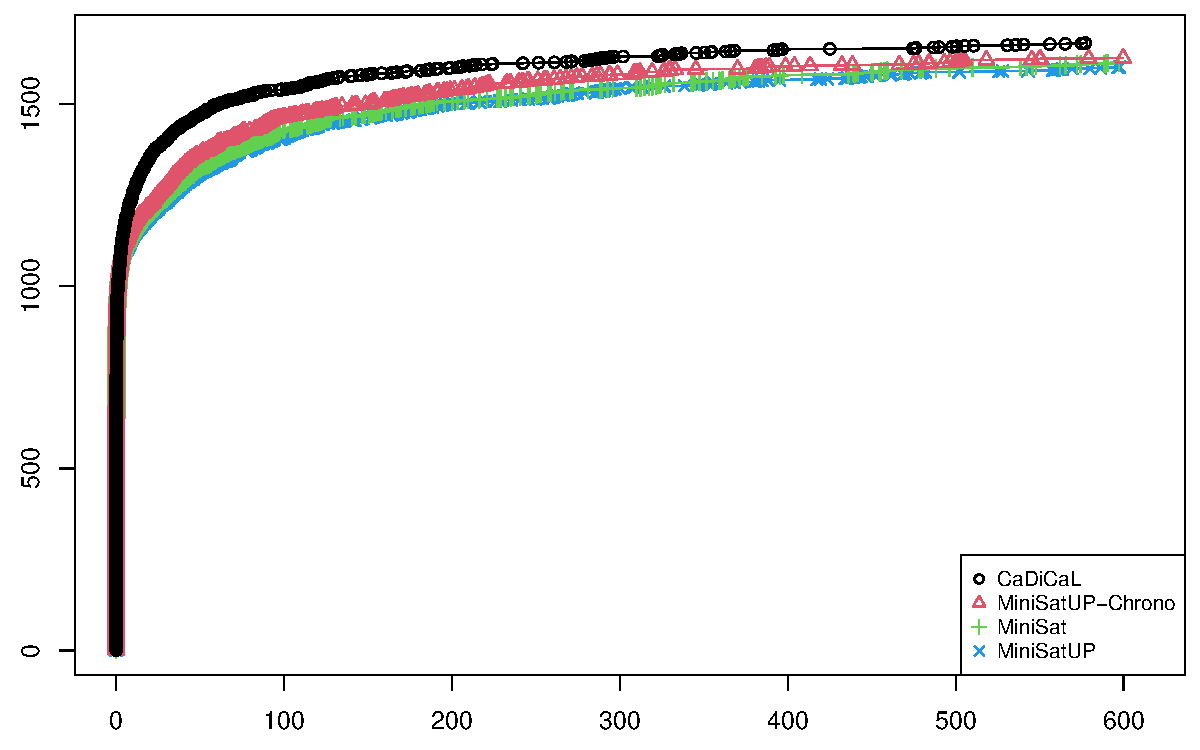
\includegraphics[width=0.85\linewidth]{plot.pdf}
    \caption{Accumulated solved instances (x-axis: running time in seconds, y-axis: number of solved instances)}
  \end{figure}
\end{frame}

\section{Summary and Future Work}

\begin{frame}{Summary}
  \begin{itemize}
    \item MiniSatUP: MiniSat extended with the IPASIR-UP interface
    \item Integrated MiniSatUP with cvc5
    \item Second implementation of IPASIR-UP after CaDiCaL
    \item Demonstrates practical, fine-grained SAT solver collaboration
    \item No performance overhead observed
  \end{itemize}
\end{frame}

\begin{frame}{Future Work}
  \begin{itemize}
    \item Investigate remaining timeout cases in cvc5 integration
    \item Extend IPASIR-UP to support CaDiCaL-specific functions (termination, learned clause/fixed variable notification, resolution proof)
    \item Further abstract and simplify the SAT solver interface in cvc5 with IPASIR-UP
    \item Support proof validation in IDRUP format for MiniSatUP
    \item Further develop and optimize MiniSatUP with chronological backtracking
  \end{itemize}
\end{frame}

\begin{frame}[t,allowframebreaks]{References}
  \scriptsize
  \nocite{*}
  \bibliographystyle{amsalpha}
  \bibliography{bibliography}
\end{frame}

\begin{frame}{Thank You}
  Questions?
\end{frame}

\end{document}
